
\section{Modelling Biases}
\label{sec:biases}

In this section, we (i) update the central bias model of \cite{clarke-tatler2014} to make use of a truncated Gaussian distribution that allows us to take the image boundaries into account. (ii) explore the strength of the leftwards bias in relation to the central bias, and (iii) describe the saccadic flow model. 


%%%%%%%%%%%%%%%%%%%%%%%%%%%%%%%%%%%%%%%%%%%%%%%%%%%%%%%%%%
\subsection{Modelling Methods}
\label{sec:modellingMethods}
%%%%%%%%%%%%%%%%%%%%%%%%%%%%%%%%%%%%%%%%%%%%%%%%%%%%%%%%%%

Here, we give an overview of the methods and data used for the saccadic flow modelling.

\subsubsection{Datasets}

We will use a number of previously published datasets, covering a range of tasks, images, and experimental set-ups. This allows us to produce a model that will generalise well to other datasets. The models will be trained on eight of the ten datasets used in \cite{clarke-tatler2014}. We chose to remove the data from \cite{asher2013} from our training set as the images have an aspect ratio of 5:4, whereas the rest of the data in our training set has an aspect ratio of 4:3. The pedestrian search dataset \citep{ehinger2009} was removed from the training set as previous analysis \citep{clarke-tatler2014} shows that it is biased compared to the other datasets analysed. Both of these datasets are now used as test sets to evaluate how well our models generalise. 

We also add four new datasets to the ten used by \cite{clarke-tatler2014}. These will be used to test the model. 

\begin{itemize}

\item \cite{jiang2014} collected data from 16 observers viewing 500 natural scenes containing crowds of people (aspect ratio 4:3).

\item \cite{clarke2009} investigated visual search for a target on a homogeneous textured background (i.e. target in noise). This dataset differs from the previous in that there is no semantic image content in the scene, and the stimuli had a 1:1 aspect ratio.

\item \cite{greene-wolfe2012} released a dataset of observers viewing square greyscale photographs.

\item \cite{borji2015} recently released a very large ($\approx 0.625$million fixations, 2000 images) dataset collected over twenty different stimuli types. Given the size of this dataset, and the wide-screen 16:9 aspect ratio, the evaluations on this dataset are presented separately, and split by stimuli class.

This gives us a relatively homogeneous training test, and a more heterogeneous test set. Hence, good performance on the test sets will likely be indicative of a generalisable result. An overview of the datasets used is given in Appendix Tables \ref{tab:datasets} and \ref{tab:setuptable}. 

\end{itemize}


\subsubsection{Pre-processing}

As with \cite{clarke-tatler2014}, normalised all fixations to the image frame, keeping the aspect ratio constant. i.e., $(x,y)\in (-1.-1)\times(-a,a)$ with typically $a=0.75$. The initial saccades after image onset ($9.1\%$ of the data) were excluded, giving us a total of 159,226 saccades. Saccades with a start or end point falling outside of the image frame were also removed. 

When fitting saccadic flow models, we \textit{mirrored} the set of fixations, by adding in horizontally and vertically reflected copies of the data. This has two advantages. (i) It is an easy way to make the saccadic flow bias symmetric in the horizontal or vertical directions. This is similar to how the central bias was defined \cite{clarke-tatler2014}. (ii) It increases the amount of data available for fitting by a factor of four. This is important as (due to the central bias) there are relatively few saccades that originate from the corners of the images. By equating all corners, we can pool the data and obtain more stable estimates for the underlying distribution. The downside of mirroring saccades in this manner is that our model of saccadic flow will be insensitive to the \textit{leftwards} bias in natural scene viewing \citep{nuthmann-matthias2014}. However, as this acocunts for a relatively small proportion of the overall variance in the data (Section \ref{sec:LeftRight}), we view this as an acceptable trade-off. Similarly, as we do not factor in the timecourse of the scanpath, we will not capture \textit{coarse-to-fine} dynamics (saccadic amplitude tends to decrease with time from stimulus onset).


\subsection{Truncated Central Bias}
\label{sec:truncatedCentral}

First, we will update the central bias from \cite{clarke-tatler2014} and use a truncated normal distribution. This is very straight forward. Re-fitting a multivariate Gaussian to the data reduces the deviance in the central bias model by $4.4\%$. Using a truncated Gaussian gives us an improvement of $12\%$. We can round the truncated Gaussian model to $\mu = (0,0)$, with a covariance matrix of $(0.32, 0; 0, 0.144)$ with no loss of precision. i.e. this is identical to \cite{clarke-tatler2014} except with $\sigma=0.32$ rather than $0.22$.

\subsection{Left v Right}
\label{sec:LeftRight}

As mentioned above, the downside of mirroring the saccades in our dataset is that our bias model will be symmetric and will be unable to exhibit the leftward bias observed in human fixation data. Here, we investigate the size of the leftwards bias by plotting how the distribution of horizontal fixation location varies with fixation number (Figure \ref{fig:leftrightDist}). We can see that while we do have a leftwards bias in our data, it is a small effect that only last for the first five fixations after scene onset. Furthermore, there is no sign of an asymmetry in the vertical direction. Fitting an ANOVA to predict the $x$-coordinates of the fixations given the fixation number gives adjusted $R^2=0.004$. If we limit our analysis to the first five fixations in each scanpath, this only increases to adjusted $R^2=0.01$. This suggests that by treating everything as symmetrical, we lose little explanatory power, while restricting the number of parameters, or increasing the amount of data available (by mirroring fixations). 

\begin{figure}
\centering
\subfigure{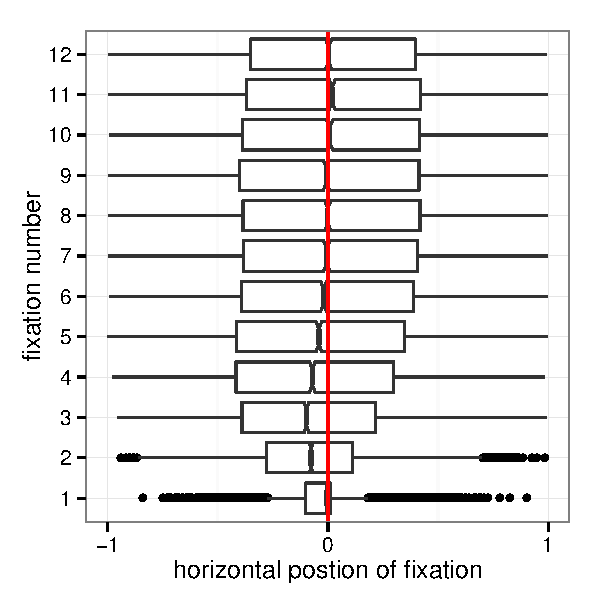
\includegraphics[width=3.8cm]{../scripts/leftVright/graphs/leftrightbias.pdf}}
\subfigure{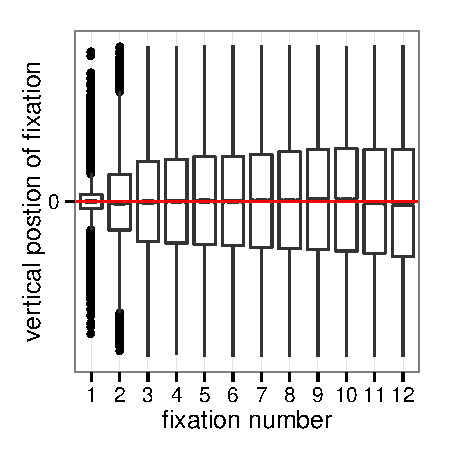
\includegraphics[width=3.8cm]{../scripts/leftVright/graphs/updownbias.pdf}}
\caption{Boxplots showing the distribution of horizontal and vertical fixations by fixation number in the merged training set}
\label{fig:leftrightDist}
\end{figure}


\subsection{Saccadic Flow}
\label{ModellingFlow}

Saccadic flow can be thought of as a generalisation of the central bias., and is illustrated in Figure \ref{fig:empiricalSaccadicFlow}. Instead of computing the distribution of all saccadic endpoints in a dataset, we look at the distribution of saccade endpoints given the start points. i.e.,for a saccade from $(x_0, y_0)$ to $(x_1, y_1)$ we want to model $p(x_1,y_1|x_0, y_0)$.

\subsubsection{Modelling}

To characterise how the distribution of saccadic endpoints varies with the start point, we used a sliding window approach. All saccades that originated from a $n\times n$ window were taken and used to fit a truncated multivariate Gaussian distribution using the \texttt{tmvtnorm} library for \texttt{R}. This window was moved in steps of $s=0.01$ from $[-1,-0.75]$ to $[1-n, a-n]$. Windows containing less than 250 datapoints were discarded. We experimented with varying the window size ($n\in\{0.05,0.1, 0.2\}$). However, as this parameter was found to have a negligible result, we only report the results for $n=0.05$.

Multivariate polynomial regression was then used to fit 4-th order polynomials to each of the parameters. As polynomial regression performs poorly in the presence of outliers, we will also use robust estimation (\texttt{rlm} from the \texttt{MASS} library). This will stop the model fits being overly influenced by outlier points from the image boundary. 

\subsubsection{Results}

Figure \ref{fig:nParamsOverSpace} shows how the parameters for the truncated multivariate Gaussian distributions vary over horizontal position for a selection of vertical positions. The regression coefficients (given in supplementary materials) allow us to estimate the conditional probability of a saccade to $(x_1, y_1)$ given the starting fixation $(x_0, y_0)$. As the robust estimation methods give a far better fit to the data, we will use this version of the model and discard the polynomial regression version.

\begin{figure*}
\centering
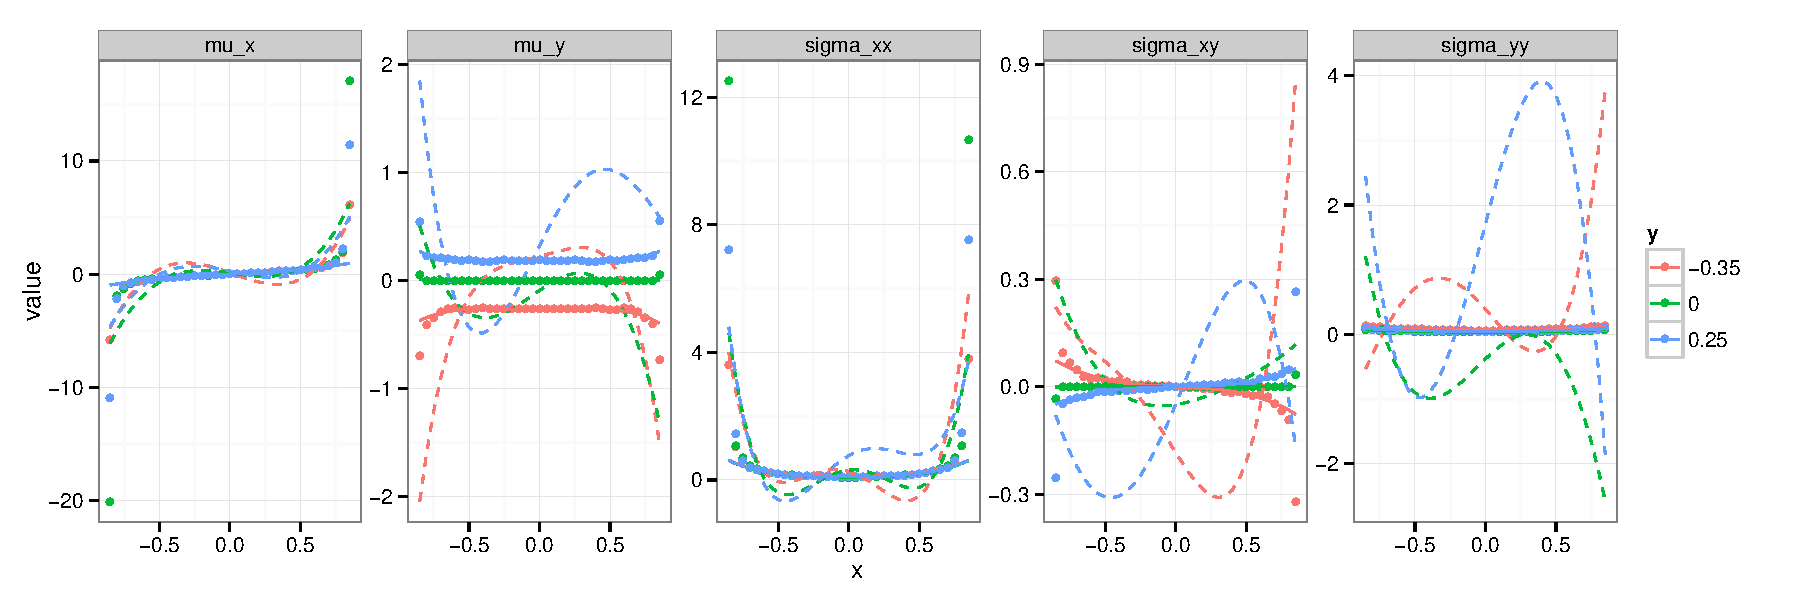
\includegraphics[width=16cm]{../scripts/flow/figs/NparamsChagingOverSpace_ALL_tN}
\caption{How the truncated Gaussian parameters vary with saccadic starting location. Dotted line show polynomial regression fits, solid line shows robust polynomial regression.}
\label{fig:nParamsOverSpace}
\end{figure*}


How well does this model account for the fixations in our datasets? Figures \ref{fig:nFlowDevAll}, \ref{fig:nFlowDevAll2} and \ref{fig:nFlowDevBorji} compared the log-likelihood of the flow model compared to the \cite{clarke-tatler2014} central baseline and a uniform distribution. We can see that in all cases, the log likelihood for the data under the flow model is higher than the central baseline and the uniform distribution. It is interesting to note that this holds even for datasets (those involving visual search) in which the central bias is outperformed (terms of log-likelihood) by the uniform distribution: chiefly the data from \cite{clarke2009,asher2013,tatler2007}. 



\begin{figure*}
\centering
 \includegraphics[width=12cm]{../scripts/flow/figs/llh_training.pdf}
\caption{Flow:normal log likelihood results. We can see that re-fitting the central-bias to each specific dataset offers little improvement over using the Clarke-Tatler model, while the flow model offers a substantial improvement.}
\label{fig:nFlowDevAll}
\end{figure*}

\begin{figure*}
\centering
\includegraphics[width=12cm]{../scripts/flow/figs/llh_testing.pdf}
\caption{Doing the same but with some new testing datasets!}
\label{fig:nFlowDevAll2}
\end{figure*}

\begin{figure*}
\centering
 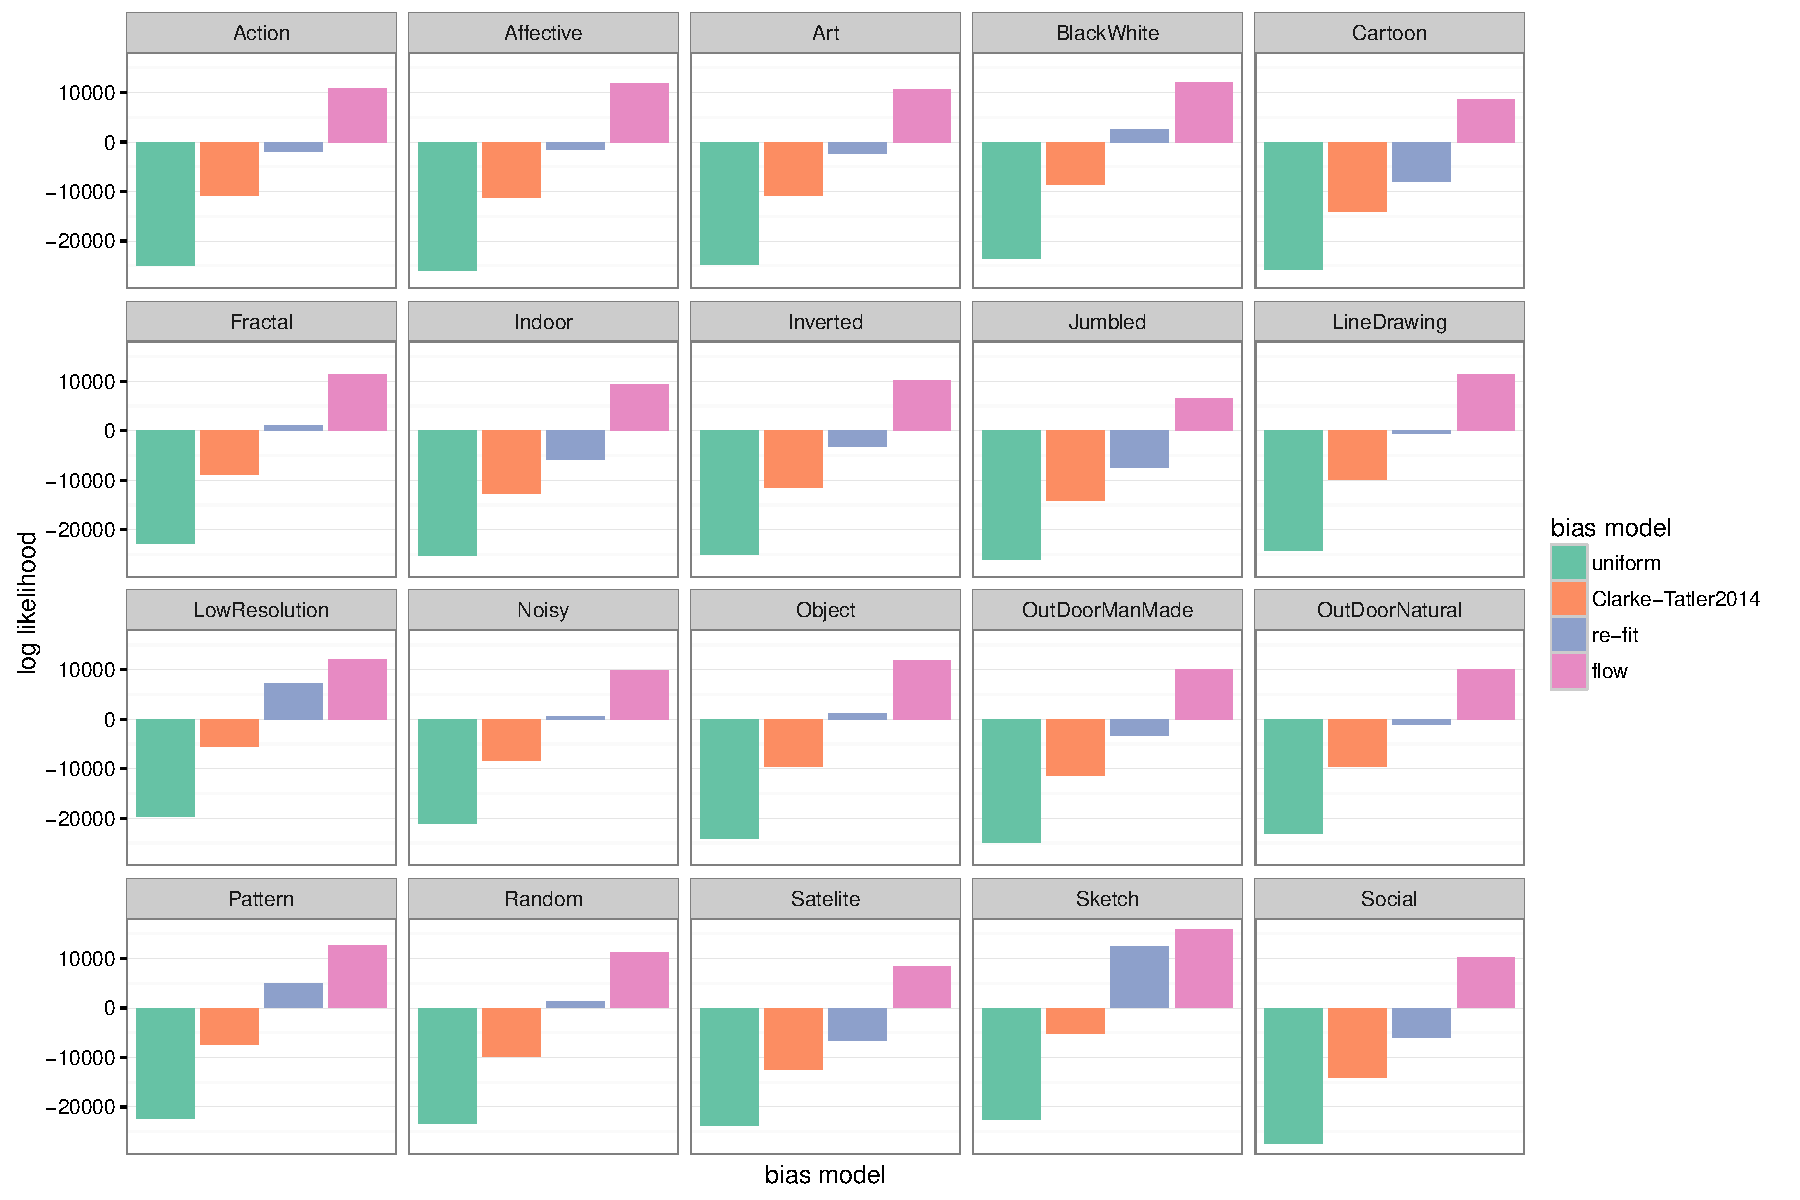
\includegraphics[width=12cm]{../scripts/flow/figs/llh_Borji.pdf}
\caption{Flow:normal deviance results. We can see that re-fitting the central-bias to each specific dataset offers little improvement over using the Clarke-Tatler model, while the flow:normal model decreases the deviance by half.}
\label{fig:nFlowDevBorji}
\end{figure*}

% \begin{figure}
% \centering
%  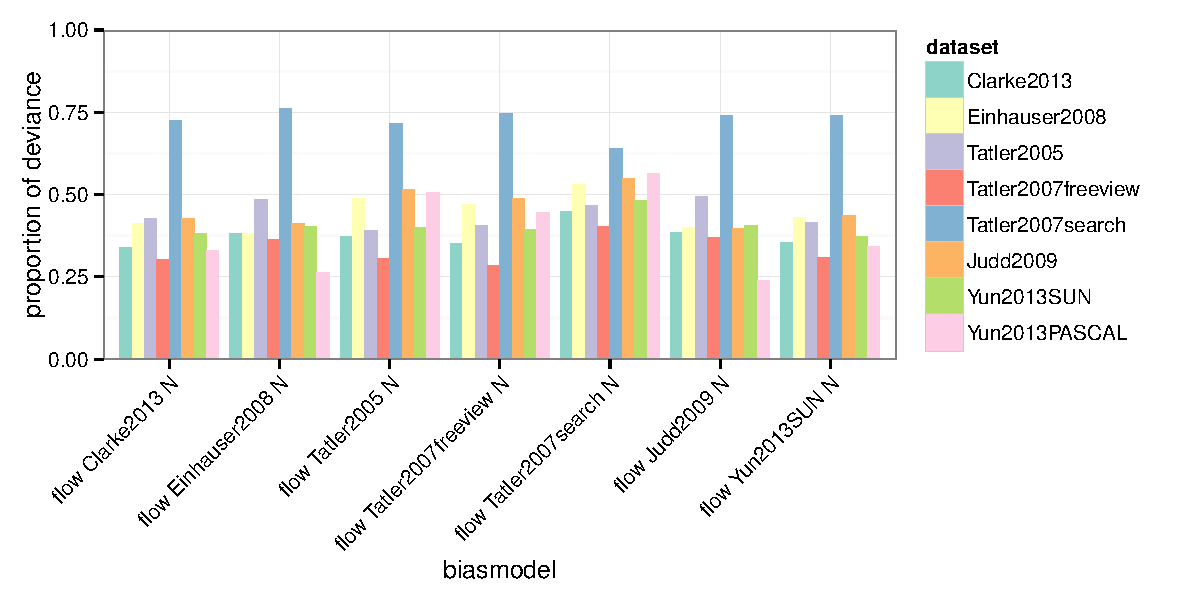
\includegraphics[width=12cm]{../scripts/flow/figs/llh_crossDataset.pdf}
% \caption{Flow:normal deviance results over datasets. In general, we can see that bias models trained on different datasets all explain around the same amount of variance in the datasets.}
% \label{fig:nFlowDevCross}
% \end{figure}